\section[Résumé détaillé en français]{Résumé détaillé}

\vspace*{1cm}

{\noindent\large\bfseries\sffamily INTRODUCTION}

Le changement climatique est une réalité incontestable. L'année 2023 en est un exemple frappant. A l'échelle mondiale, la température moyenne annuelle a dépassé les températures mesurées depuis 1850 (\Cref{fig:R1}), et a probablement été l'année la plus chaude des 2000 dernières années \citep{Esper2024}. L'augmentation continue des concentrations atmosphériques de dioxyde de carbone (atteignant 419 ppm en 2023), provoquée par les activités humaines, est au moins en partie responsable de ces évènements extrêmes. 

\begin{figure}
\vspace*{-0cm}
\centering
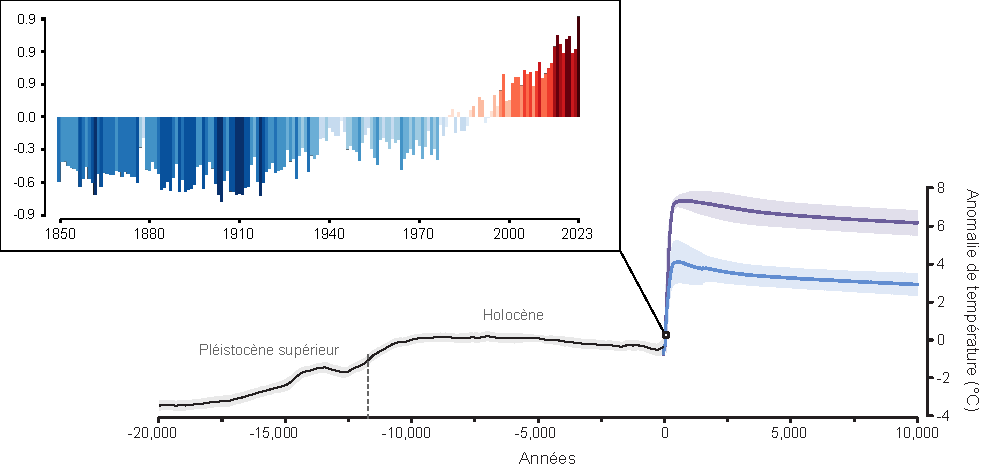
\includegraphics{resume/figs/clark2016_climatestrips_FR.pdf}
\caption{\textbf{Changements passés et futurs des températures globales.} Le graphique principal est une adaptation de la figure dans \citet{Clark2016}, et montre la température (moyenne$\pm$écart-type) reconstituée à partir d'archives paléoclimatiques depuis 20.000 ans et selon des simulations réalisées avec les modèles UVic et Bern3D-LPX pour les prochains 10.000 ans, pour deux scénarios d'émission différents (bleu: 2,560 PgC, violet: 5,120 PgC). Le cadre supérieur montre la dynamique récente (1850-2023) selon le jeu de données HadCRUT5 (UK Met Office), en reprenant la charte graphique créée par \href{https://showyourstripes.info/}{Ed Hawkins}.}
\vspace*{-0cm}
\label{fig:R1}
\end{figure}

La Terre a toujours alterné entre des périodes chaudes et des périodes glaciaires - nous sommes actuellement dans la glaciation du Quaternaire qui a commencé il y a 2,58 millions d'années. Tout au long du Quaternaire, plusieurs cycles glaciaires et interglaciaires se sont également succédés \citep{Snyder2016, Koehler2010}. Le dernier événement majeur de réchauffement climatique a été la transition entre le dernier maximum glaciaire (il y a 21 000 ans) et le début de la période interglaciaire que nous connaissons actuellement (il y a 11 700 ans ; \Cref{fig:R1}). Cette période, appelée Holocène, est caractérisée par des conditions climatiques chaudes et stables qui ont permis à la civilisation humaine de prospérer, notamment grâce au développement de l'agriculture. 
Cependant, l'étude du climat passé nous montre également qu'au cours des 50 dernières années, les activités humaines ont réchauffé le climat à un rythme sans précédent depuis au moins 2000 ans. De nombreux indicateurs climatiques sont à des niveaux jamais atteints depuis des siècles, voire des millénaires, et nous observons déjà des impacts importants sur toutes les composantes de la biosphère \citep{IPCC2021}.

Le climat est en effet l'un des principaux moteurs de la dynamique des écosystèmes et affecte de nombreux processus écologiques. Par exemple, les aires de répartition de nombreux organismes terrestres se déplacent en réponse au réchauffement climatique, généralement vers des latitudes et des altitudes plus élevées, c'est-à-dire vers des conditions plus fraîches \citep{Lenoir2008, Elmendorf2015, Pecl2017, Vitasse2021, Rumpf2018, Zurell2024}. Les forêts ne sont pas épargnées par ces changements importants. 
Les fluctuations climatiques passées ont induit des changements de végétation à grande échelle \citep{Hoogakker2016, Nolan2018}, et notamment déclenché des extinctions majeures \citep{Svenning2003}.  Au cours du dernier épisode de réchauffement du début de l'Holocène, les arbres ont migré depuis des refuges glaciaires vers des terrains précédemment recouverts de glace \citep{Brewer2002, TerhuerneBerson2004, Saltre2013, Robin2016}. Ces dynamiques ont largement contribué à façonner les forêts que nous connaissons aujourd'hui, à la fois en termes de diversité spécifique \citep{Svenning2007} et de diversité génétique \citep{Cheddadi2006}.

Aujourd'hui, les conditions climatiques plus chaudes et plus sèches que la moyenne ont un impact important sur les écosystèmes forestiers \citep{Allen2010, Senf2020}. En Europe, les sécheresses ont été responsables d'une surmortalité forestière de 500.000 hectares entre 1987 et 2016 \citep{Senf2020}. Cette mortalité peut survenir de différentes façons : soit directement à cause de la sécheresse (dégradation de l'état hydrique de la plante; \citealp{Hartmann2018}), soit à cause d'une vulnérabilité accrue aux épidémies d'agents pathogènes et aux incendies à grande échelle \citep{Breshears2005, Seidl2017, Sommerfeld2018, Jactel2012, Mantgem2009, Hember2016}. Ces perturbations forestières généralisées ont des conséquences durables quant aux rétroactions du cycle du carbone sur le changement climatique \citep{Schwalm2012, Ciais2005, Thom2016, Kannenberg2020, Kurz2008}. Elles limitent le potentiel des forêts à atténuer le changement climatique \citep{Anderegg2020}. Il est donc urgent de mieux comprendre comment les forêts réagissent au changement climatique et l'influencent -- d'autant plus que nos émissions de carbone auront des conséquences pour les siècles (voire les millénaires) à venir (\Cref{fig:R1}).

Les modèles sont des outils critiques pour mieux appréhender les interactions entre la forêt et le climat. Ils permettent notamment d'étudier des phénomènes à grande échelle, difficiles ou impossibles à tester expérimentalement (par exemple, la répartition d'une espèce sur un continent). Ils sont aussi souvent utilisés pour prédire le comportement des écosystèmes dans de nouvelles conditions (par exemple dans des conditions climatiques futures). En particulier, pour comprendre les processus écologiques impliqués dans la distribution géographique des espèces, les écologues utilisent principalement des modèles empiriques (phénoménologiques, statistiques, corrélatifs) et des modèles basés sur des processus (mécanistes, de simulation).

La grande majorité des études utilise des modèles empiriques. Nous les appellerons CSDMs ci-dessous, pour \emph{correlative species distribution models}. Ils sont basés sur des relations statistiques entre les occurrences observées des espèces et des prédicteurs environnementaux \citep{Elith2009}, principalement des variables climatiques (c'est-à-dire des moyennes de variables mensuelles calculées sur une période standard de 30 ans). Ces approches ont considérablement évolué, de la régression statistique \citep{Thuiller2009} aux modèles d'intelligence artificielle utilisant des dizaines de variables \citep{Steiner2024}. Cependant, ces modèles sont de plus en plus critiqués: les relations statistiques significatives peuvent en effet résulter d'une simple corrélation entre les variables explicatives et les distributions d'espèces plutôt que d'une relation causale réaliste \citep{Bahn2007, Journe2020, Fourcade2018}.

Parallèlement, des modèles basés sur les processus ont été développés. Nous les appellerons PEMs dans les paragraphes suivants, pour \emph{process-explicit models}. Les PEMs visent à simuler les principaux processus qui régissent le fonctionnement des espèces, en s'appuyant sur des équations mathématiques explicites dont les paramètres ont une interprétation biologique directe \citep{Dormann2012}. Les PEMs peuvent fonctionner à différentes échelles, du gène à l'écosystème \citep{Pilowsky2022}. 
Les valeurs des paramètres peuvent être estimées à l'aide d'observations sur le terrain ou de données expérimentales, ou sont déjà disponibles dans la littérature. Certains paramètres peuvent être calibrés en utilisant des méthodes de modélisation inverse et des données relatives aux processus modélisés. Classiquement, les PEMs n'utilisent donc pas de données sur la présence des espèces (contrairement aux CSDMs). Leur calibration est souvent compliquée, et ne peut être réalisée pour beaucoup d'espèces.
Le développement d'un PEM est semé d'embûches : un processus peut être représenté avec une mauvaise fonction mathématique (\Cref{fig:pbmissuesA}), un processus important peut manquer dans le modèle (\Cref{fig:pbmissuesC}), les valeurs de paramètres peuvent être erronées (\Cref{fig:pbmissuesB}), ou certaines peuvent se compenser sans que l'on puisse s'en rendre compte (\Cref{fig:pbmissuesD}).

\begin{figure}
\vspace*{-0cm}
\centering
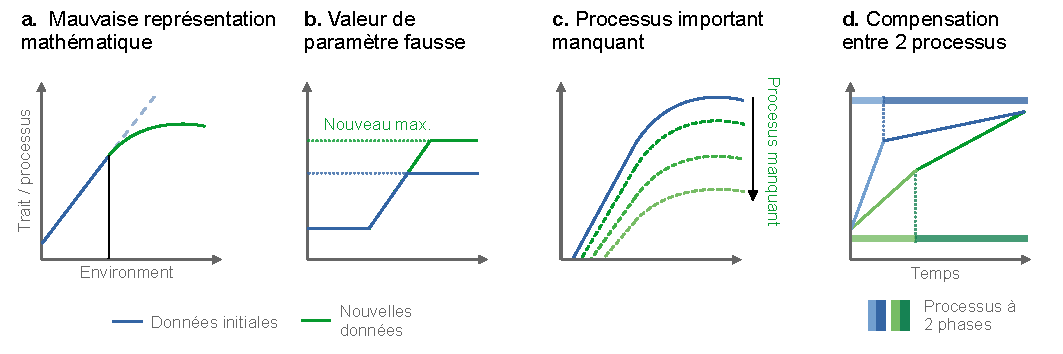
\includegraphics{resume/figs/pbm_issue_FR.pdf}
\caption{\textbf{Les différents types d'erreur qui peuvent impacter les modèles basés sur les processus.}}
\vspace*{-0cm}
\label{fig:R2}
\end{figure}

Il existe donc de multiples sources d'incertitudes et autant de possibilités d'avoir des modèles qui ne sont pas fiables. Pourtant, face à l'accélération du changement climatique, les gestionnaires de milieux naturels ont un besoin urgent de projections fiables des changements d'aires de répartition des espèces à l'échelle de leur territoire et au-delà. Les CSDMs fournissent des projections alarmantes sur l'avenir des forêts européennes \citep{Thurm2018, Dyderski2018, Chakraborty2021, Wessely2024, Mauri2022}. Le nombre d'espèces d'arbres forestiers capables de survivre par kilomètre carré devrait être réduit d'un tiers d'ici la fin du siècle \citep{Wessely2024}. Nous n'avons cependant aucune garantie que les relations statistiques des CSDMs sont causales et qu'elles se vérifieront dans les conditions climatiques futures, en dehors de la gamme de variations dans laquelle elles ont été établies \citep{Maguire2016, Fitzpatrick2018}. 
A l'inverse, les PEMs sont supposés pouvoir fournir des projections plus robustes dans des conditions climatiques nouvelles \citep{Evans2012, Connolly2017, Urban2016, Pilowsky2022}. Il s'agit d'une hypothèse séduisante car les PEM prennent plus de temps à développer, de sorte que nous pouvons espérer que ces efforts en valent la peine. Cependant, elle n'a jamais été vérifiée, et rien n'empêche les PEMs de donner des bons résultats pour de mauvaises raisons.

Les projections entre les CSDMs et les PEMs divergent fortement : ces derniers simulent généralement des taux d'extinction d'espèces plus faibles en réponse au changement climatique \citep{Morin2009, Kearney2010, Cheaib2012, Gritti2013}. La confiance dans les projections des modèles restera cependant limitée tant que nous ne pourrons pas déterminer dans quelle mesure les modèles sont transférables en dehors du contexte dans lequel ils ont été construits et calibrés - et \emph{in fine} vérifier que les modèles sont adaptés à l'objectif spécifique de réaliser des projections dans les climats futurs. Il est donc urgent d'évaluer de façon précise les performances de ces différents modèles, pour savoir quelle approche pourrait fournir des projections fiables dans le futur. En particulier, il est nécessaire d'identifier les origines de leur robustesse, et si elle réside plutôt :
\begin{itemize}
\item dans la différence entre les relations statistiques des CSDMs et les équations explicites des PEMs;
\item ou dans la différence entre la méthode d'estimation des paramètres, qui implique (CSDM) ou n'implique pas (PEM) la distribution des espèces (soit  ce que l'on essaye de modéliser). 
\end{itemize}
L'objectif général de ce travail de doctorat est donc d'évaluer la robustesse et l'incertitude des projections de la distribution future des arbres forestiers. Pour ce faire, le travail est structuré en quatre chapitres.

\begin{figure}
\vspace*{-0cm}
\centering
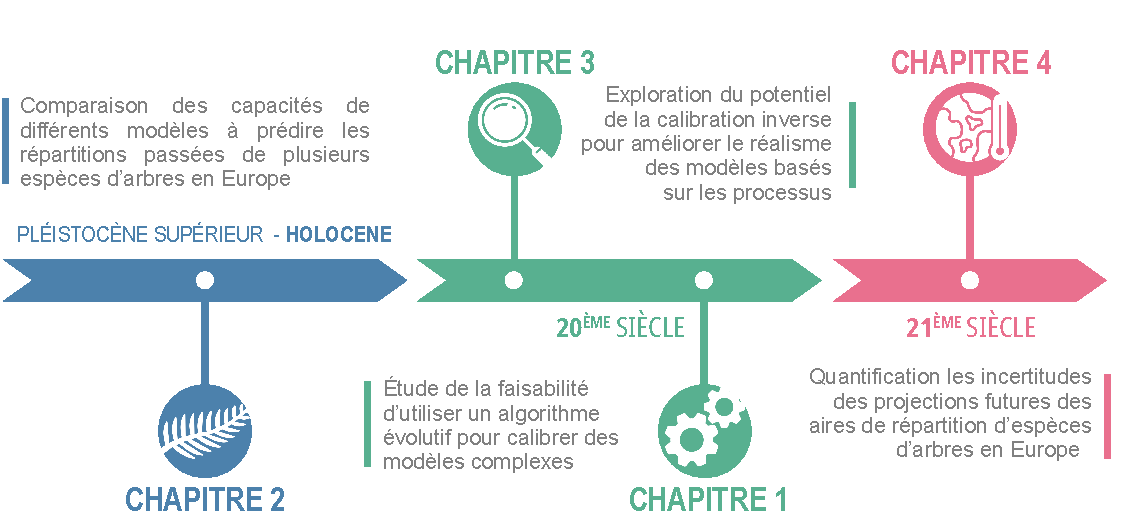
\includegraphics{resume/figs/timeline_FR.pdf}
%\caption*{\textbf{The timeline of this PhD thesis.}}
\vspace*{-0cm}
% \label{fig:R3}
\end{figure}

\clearpage

{\noindent\large\bfseries\sffamily CHAPITRE 1}

La première étape de cette thèse a été d'explorer s'il était réalisable de calibrer des PEMs complexes (avec entre 30 et 80 paramètres) en utilisant les mêmes données que les CSDMs. L'objectif était notamment de développer une approche de modélisation hybride, décrivant de façon explicite les processus tout en étant calibrée à partir des observations actuelles de la répartition des espèces. 

Nous nous sommes intéressés en particulier à deux modèles. Le premier, PHENOFIT, est un modèle de distribution des espèces (basé sur les processus) développé pour les arbres forestiers et qui se concentre sur la phénologie. Il repose sur le principe selon lequel la distribution d'un arbre dépend principalement de la synchronisation de son développement avec les conditions climatiques locales \citep{Chuine2001}. Le second, CASTANEA, est un modèle écophysiologique qui simule les flux de carbone et d'eau dans les forêts \citep{Dufrene2005}. Il est beaucoup plus complexe que PHENOFIT et modélise de nombreux processus. 

Pour ce chapitre, nous avons dû adapter un algorithme d'optimisation, appelé CMA-ES (pour \emph{covariance matrix adaptation - evolution strategy}), reconnu pour son efficacité \citep{Hansen2001, Hansen2006}, mais jamais utilisé en écologie à notre connaissance. Cet algorithme est inspiré des principes de la biologie évolutive, via la recombinaison, la mutation et la sélection des jeux de paramètres les plus adaptés (c'est-à-dire fournissant les meilleures prédictions). Afin de pouvoir réaliser les calculs en parallèle, nous avons implémenté CMA-ES sur deux clusters de calcul : GenOuest de l'IRISA-INRIA (\href{https://www.genouest.org}{genouest.org}) et TGCC (\emph{Très Grand Centre de Calcul}) du CEA (\href{http://www-hpc.cea.fr/fr/complexe/tgcc.htm}{hpc.cea.fr}). Une calibration de PHENOFIT prend ainsi environ 1 jour, alors qu'une calibration de CASTANEA dure entre 10 et 20 jours. Nous avons réalisé ces calibrations plusieurs fois pour trois espèces: le hêtre (\emph{Fagus sylvatica}), le chêne vert (\emph{Quercus ilex}) et le sapin blanc (\emph{Abies alba}).

Nos résultats ont montré que CMA-ES est un algorithme d'optimisation efficace pour la calibration inverse de PEMs complexes. L'algorithme a été capable de trouver des jeux de paramètres qui améliorent significativement la performance (mesurée ici avec une métrique classique, l'AUC) des PEMs ajustés par rapport à la paramétrisation classique.  
La calibration inverse de PHENOFIT permet ainsi une augmentation moyenne de 17,2\% de l'AUC pour les trois espèces par rapport à la calibration experte. L'augmentation maximale est obtenue pour le sapin blanc, passant de 0,72 à 0,9 (25\%). La calibration inverse de CASTANEA permet une augmentation moyenne de 23,7\% de l'AUC par rapport à la calibration experte, et une augmentation maximale est obtenue pour le chêne vert (34,7\%, \Cref{fig:R3}).

Cependant, notre étude a également mis en évidence le problème de non-identifiabilité des valeurs des paramètres. Les répétitions des calibrations ont ainsi donné des valeurs de paramètres divergentes. Les données d'occurrence ne comportent pas suffisamment d'information pour calibrer tous les paramètres simultanément, et il peut également y avoir des compensations entre les processus modélisés. Nous creuserons cet aspect dans le Chapitre 3.

\clearpage

\begin{figure}
\vspace*{-0cm}
\centering
\hspace*{-0.8cm}
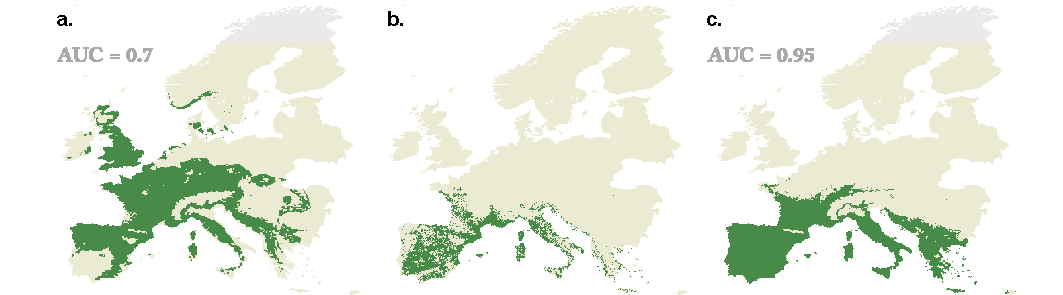
\includegraphics[width = 21cm]{resume/figs/cmaes_FR.pdf}
\caption{\textbf{Cartes de répartition du chêne vert obtenue avec la version classique de CASTANEA \textbf{(a)} et la version ajustée \textbf{(c)}, par rapport à la répartition actuelle \textbf{(a)}.}}
\vspace*{-0cm}
\label{fig:R3}
\end{figure}

Pour conclure, la calibration inverse des PEMs, en utilisant des données à large échelle comme les données de distribution, peut offrir une nouvelle perspective pour étendre l'utilisation de PEMs et faciliter leur utilisation \citep{Higgins2020, Evans2016}. La calibration de ces PEMs ajustés était un également pré-requis pour le chapitre suivant.


\vspace*{1cm}
{\noindent\large\bfseries\sffamily CHAPITRE 2}

La deuxième étape de cette thèse de doctorat consistait à fournir pour la première fois une évaluation simultanée de la transférabilité des CSDMs, des PEMs ajustés et des PEMs classiques dans des conditions climatiques très différentes. Nous avons réalisé des simulations sur les 12 000 dernières années, et comparé les résultats des modèles aux données de fossiles de pollen qui nous donnent une idée de la répartition des arbres dans le passé en Europe. L'utilisation de ces trois types de modèle nous a permis d'étudier les facteurs importants qui favorisent la robustesse des projections. En particulier, la comparaison entre les CSDMs/PEMs ajustés et les PEMs classiques nous a permet déterminer si les différences de performance des modèles proviennent de leurs méthodes de calibration (utilisant des données d'occurrence d'espèces ou non), tandis que la comparaison entre les CSDMs et les PEMs classiques/ajustés permet de déterminer si les différences de performance des modèles proviennent des hypothèses des modèles (relations décrivant des mécanismes biologiques explicites ou non).

En plus des deux PEMs mentionnés au chapitre 1, que nous avons utilisés à la fois dans leur version classique et dans leur version ajustée, nous avons sélectionné cinq modèles corrélatifs sur la base de la comparaison approfondie des modèles effectuée par \cite{Valavi2022}: GLM, GAM, BRT, MaxEnt et Random Forest. Nous avons calibré ces modèles pour cinq espèces : \textit{Fagus sylvatica} L., \textit{Abies alba} Mill., \textit{Quercus robur} L., \textit{Quercus petraea}  (Matt.) Liebl. et \textit{Quercus ilex} L. 

En termes de données climatiques, nous avons utilisé les simulations du modèle HadCM3B-M2.1 \citep{Armstrong2019}, à partir de 18.000 ans à une résolution spatiale de 0,5\degree. Pour ce travail, plusieurs variables ont été produites : la température journalière moyenne, les températures journalières minimales et maximales, les précipitations, le nombre de jours de pluie, la nébulosité et la vitesse du vent. Pour pouvoir utiliser les PEMs, nous avons ensuite généré des données quotidiennes avec le générateur météorologique GWGEN \citep{Sommer2017}, pour des périodes de 30 ans tous les 250 ans. Nous avons également simulé le rayonnement solaire extra-terrestre quotidien avec les mêmes conditions de forçage orbital utilisées dans HadCM3B-M2.1 \citep{Armstrong2019}, puis nous avons calculé le rayonnement global quotidien comme dans le modèle LPJ-LMfire \citep{Pfeiffer2013}. 

A partir des projections de la répartition des espèces, nous avons également pris en compte la migration des espèces au cours du temps grâce à un simple automate cellulaire \citep{Engler2012} à une résolution de 500 m. Nous avons fait commencer ces simulations à partir de 12 000 ans (ou 11 750 lorsqu'un modèle ne simulait aucune présence à 12 000 ans). Nous n'avons pas pu commencer plus tôt (par exemple, à partir de 15 000 ans), car la plupart des modèles ne simulaient aucune présence autour de 12 500 ans.

Nous avons enfin quantifié la dissimilarité entre le climat de l'Holocène, le climat historique (1901-2000) et le climat futur. Pour cela, nous avons défini le climat dans chaque période grâce à un hypervolume en trois dimensions, représentant les trois premiers axes d'une ACP réalisée à partir des moyennes des températures sur trois mois et des sommes des précipitations sur trois mois. Pour caractériser les conditions climatiques futures, nous avons utilisé 34 modèles climatiques \citep{Thrasher2022} et 2 scénarios socio-économiques (SSP2-4.5 et SSP5-8.5).

\begin{figure}
\vspace*{-0cm}
\centering
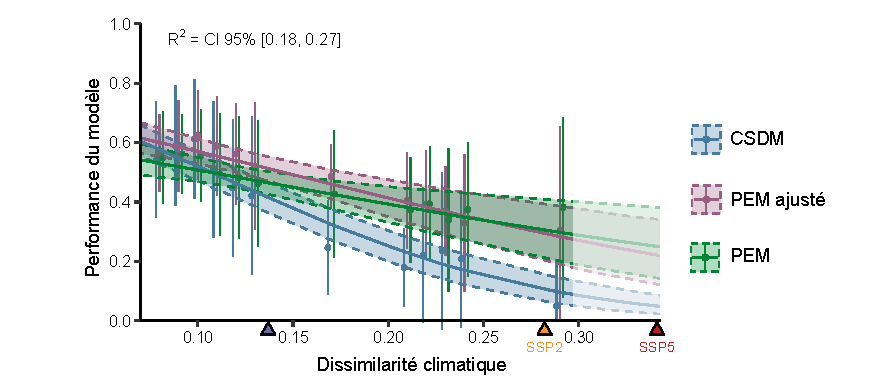
\includegraphics{resume/figs/pastperformance_FR.pdf}
\caption{\textbf{Performance des différents modèles en fonction de la dissimilarité climatique}. La droite correspond à une régression bayésienne Bêta, avec l'intervalle de crédibilité à 95\%. Les points représentent la performance moyenne du modèle (et les lignes associées représentent l'écart type). Le triangle bleu sur l'axe des abscisses représente la limite entre le début de l'Holocène ($>$ 8.200 années) et le milieu et la fin de l'Holocène ($<$ 8.200 années). Les triangles jaunes et rouges représentent le niveau potentiel de dissimilarité climatique en 2060 pour les deux scénarios futurs.}
\vspace*{-0cm}
\label{fig:R4}
\end{figure}

Les performances de tous les modèles diminuent lorsque l'on s'éloigne dans le passé, c'est-à-dire dans des conditions climatiques de plus en plus différentes des conditions historiques (\Cref{fig:R4}). Cependant, la diminution de performance des PEMs (classiques ou ajustés) est moins importante que la diminution de performance des CSDMs. En particulier, les PEMs ont une meilleure transférabilité dans les conditions climatiques les plus éloignées (du début de l'Holocène) que les CSDMs. Nos résultats ont également révélé que la calibration inverse des PEMs améliore leur performance dans le passé récent sans toutefois altérer de manière significative leur transférabilité à long terme (\Cref{fig:R4}).

Nos résultats démontrent donc, pour la première fois, que notre compréhension des mécanismes biologiques intégrés dans les PEMs pourraient représenter un réel avantage par rapport aux relations empiriques utilisées dans les CSDMs pour augmenter la fiabilité des projections des modèles dans des conditions climatiques très différentes. En particulier, nos résultats semblent montrer que les processus explicitement représentés dans les modèles sont plus importants que la méthode de calibration. Ils suggèrent également que les prévisions des PEMs, classiques ou ajustés, devraient être plus fiables au moins jusqu'en 2060 (selon le scénario SSP245).

\vspace*{1cm}
{\noindent\large\bfseries\sffamily CHAPITRE 3}

Dans ce chapitre, nous souhaitions comprendre plus en détail dans quelle mesure la calibration inverse pouvait vraiment favoriser l’utilisation des PEMs pour un plus grand nombre d’espèces. En particulier, nous avons examiné si la structure des PEMs contraignait suffisamment la calibration -- ce qui est généralement supposé \citep{Higgins2020} -- et dans quelle mesure les PEM ajustés pouvaient simuler des processus réalistes. 

Pour ce faire, nous nous sommes concentrés sur la calibration de PHENOFIT, à partir des données de distribution \citep{VanderMeersch2023}. Nous avons d’abord examiné en détail 100 calibrations obtenues pour le hêtre (\emph{Fagus sylvatica} L.), en évaluant le réalisme des processus simulés par rapport à des observations phénologiques dans toute l’Europe et en analysant les compensations entre les paramètres. Nous avons ensuite cherché à évaluer si la calibration inverse pouvait améliorer l’estimation de la valeur de certains paramètres pour lesquels des données précises sont rares.

Pour ce deuxième point, nous avons effectué des calibrations inverses pour sept espèces différentes (\emph{Abies alba},  \emph{Betula pendula}, \emph{Fagus sylvatica}, \emph{Fraxinus excelsior}, \emph{Larix decidua}, \emph{Picea abies},  \emph{Quercus pubescens} et \emph{Quercus robur}). Nous avons calibré uniquement les paramètres qui correspondaient à des processus que nous avons identifiés comme responsables des erreurs de la version classique du modèle.

Nos résultats montrent que la calibration inverse des PEMs à l’aide de données de distribution des espèces ne conduit pas nécessairement à des paramètres réalistes. Ainsi, nous avons obtenu des erreurs importantes sur les dates phénologiques simulées avec les jeux de paramètres ajustés pour le hêtre. Nous avons également mis en évidence des compensations entre les processus. Par exemple, on distingue deux grands groupes de calibration pour le débourrement : un premier groupe avec une phase d'endodormance courte et une phase d'écodormance longue, qui avait une erreur médiane de 28,3 jours pour la date de débourrement et un second groupe avec une phase d'endodormance longue et phase d'écodormance courte avec une erreur médiane plus faible de 16,3 jours.

Nos résultats démontrent également que la calibration inverse peut être très utile pour calibrer certaines parties d’un modèle lorsque des données spécifiques font défaut \citep{Evans2016}. Par exemple, pour plusieurs espèces, la calibration du modèle de maturation des fruits a permis d'augmenter la performance du modèle et de simuler des dates de maturation plus réalistes en moyenne. 

Dans l’ensemble, la calibration inverse est une méthode prometteuse. Cependant, les équations mathématiques des PEMs qui décrivent explicitement certains mécanismes ne contraignent pas suffisamment le processus de calibration. Il faut donc nécessairement une évaluation approfondie des résultats pour s'assurer de simuler des processus réalistes.

\vspace*{1cm}
{\noindent\large\bfseries\sffamily CHAPITRE 4}

Il existe un besoin crucial de projections fiables pour appuyer la prise de décisions, avec une quantification robuste des incertitudes. Le dernier objectif de cette thèse était de produire des projections futures des changements d'aire de répartition des espèces d'arbres forestiers d'Europe, selon différents scénarios, en utilisant les modèles mobilisés dans les chapitres précédents (CSDM, PEM ajusté et PEM).

Les simulations futures ont été effectuées avec les dernières projections climatiques de CMIP6. Nous avons sélectionné cinq modèles climatiques, et 2 scénarios (SSP2 et SSP5). La résolution des projections a été augmentée à 0.1\degree grâce à une méthode statistique de \emph{downscaling} préservant les tendances \citep{Noel2022}. Nous avons effectué ces simulations pour six espèces : \emph{Abies alba} Mill., \emph{Fagus sylvatica} L., \emph{Quercus petraea} (Matt.) Liebl., \emph{Quercus robur} L., \emph{Quercus pubescens} Willd. et \emph{Quercus ilex} L.

Pour quantifier les incertitudes, nous nous sommes initialement inspirés des approches élaborées par Hawkins et Sutton \citep{Hawkins2009, Hawkins2011}. Pour estimer l'importance relative des incertitudes liées aux modèles de distribution (SDM), aux scénarios climatiques (SSP), aux modèles climatiques (GCM) et aux différentes espèces considérées, nous avons décomposé la variance grâce à une ANOVA (en prenant en compte les effets d'interaction entre les différents facteurs). Nous avons effectué des ANOVA pour toutes les espèces simultanément, et pour chaque espèce séparément. Nous avons divisé l'Europe en cinq écorégions : Méditerranéenne, Atlantique, Continentale, Alpine et Boréale. 

Pour toutes les espèces confondues, les différences entre les réponses des espèces étaient la principale source d’incertitude pour les écorégions Atlantique et Continentals (respectivement 56,6\% et 42,4\% de l'incertitude totale des projections en 2090). La différence entre les SDMs était la première source d'incertitude dans la région Boréale (33.7\%), et la seconde dans la région Continentale (29.4\%). 

Au niveau des espèces, la plus grande incertitude découle de l’écart entre les projections des différents SDMs. À l’exception de la région Alpine, cela représente la principale source d’incertitude pour les quatre autres écorégions (entre 54,2\% et 64,8\%). Par exemple, dans l’écorégion Continentale, les différences entre les SDMs représentent 73,7\% de l’incertitude totale des projections pour le hêtre. 

Nos résultats ont donc montré que les différences entre les types de SDMs sont responsables d'une part importante des incertitudes des projections futures. Les projections des CSDMs et PEMs sont en effet connues pour diverger de manière significative \citep{Morin2009, Keenan2011a, Cheaib2012, Takolander2019}. Dans ce chapitre, nous avons montré pour la première fois que les projections très pessimistes dans le Sud et le Sud-Ouest de l'Europe sont associées à la méthode de calibration utilisée. En effet, les deux approches de modélisation -- CSDM ou PEM -- calibrées à partir des données actuelles d'occurrence des espèces prédisent des extinctions plus importantes à la limite sud de l’aire de répartition des espèces que les PEMs classiques (\Cref{fig:R5}). Il est intéressant de noter que les PEMs ajustés présentent un comportement intermédiaire entre les CSDMs et les PEMs classiques, car ils projettent également une augmentation importante des conditions favorables dans le Nord et l'Est de l'Europe, comme les PEMs classiques (\Cref{fig:R5}).

\begin{figure}
\vspace*{-0cm}
\centering
\hspace*{-1.2cm}
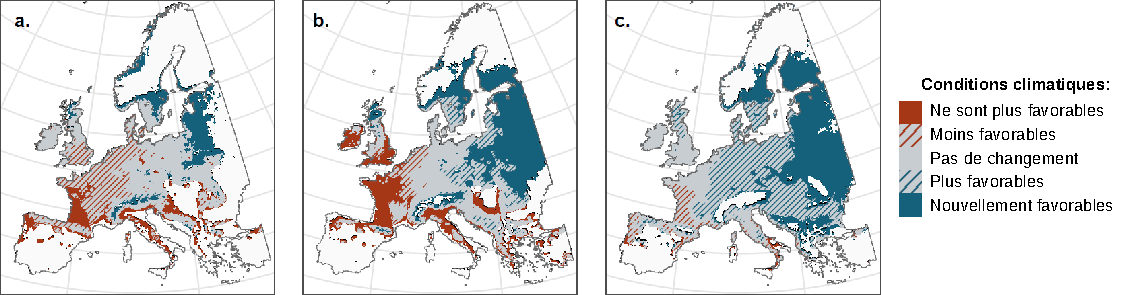
\includegraphics[width = 20cm]{resume/figs/fagus_FR.pdf}
\caption{\textbf{Projections de l'aire de répartition du hêtre en 2090, selon (a) des CSDM (b) des PEMs ajustés (c) des PEMs classiques.}}
\vspace*{-0cm}
\label{fig:R5}
\end{figure}

Au-delà des différences entre les approches de modélisation, les projections multi-modèles sont particulièrement utiles pour identifier des tendances générales et orienter la gestion forestière. Nos résultats soulignent qu'il est essentiel de tenir compte de la diversité des approches de modélisation existantes afin d’assurer une quantification robuste de toutes les incertitudes, pour éviter un excès de confiance dans les projections des modèles \citep{Simmonds2024}. 

\vspace*{1cm}
{\noindent\large\bfseries\sffamily DISCUSSION} 

Notre évaluation de la transférabilité des modèles au cours des 12 000 dernières années nous porte à croire qu'une description explicite des processus comme dans les PEMs est essentielle pour améliorer la performance des modèles, contribuant ainsi à une plus grande robustesse des modèles aux changements climatiques majeurs. À la fin du Pléistocène/début de l’Holocène, les modèles basés sur les processus apparaissaient meilleurs pour prédire les refuges climatiques -- les endroits où les espèces auraient pu survivre dans des conditions climatiques très différentes.
Cela semble vrai à la fois pour les PEMs classiques (dont les valeurs des paramètres ne dépendent pas de la distribution actuelle) et les PEMs ajustés (calibrés de la même manière que les CSDMs). Nous avons ainsi démontré pour la première fois qu'il y a un réel avantage, pour améliorer la transférabilité du modèle, à traduire nos connaissances sur le fonctionnement des espèces en équations mathématiques qui supposent, \emph{a priori}, des relations causales entre les conditions climatiques et les mécanismes simulés. 

Cependant, nous avons aussi montré que la calibration inverse des PEMs ajustés peut conduire à des processus totalement irréalistes. Par exemple, nous avons obtenu des erreurs significatives dans les processus phénologiques, en perdant ainsi les avantages des PEMs. Le fait que les PEMs ajustés semblent assez fiables dans le passé lointain malgré des paramètres irréalistes met en évidence qu’il est possible d’obtenir des résultats corrects pour de mauvaises raisons, même dans des conditions climatiques très différentes (c'est-à-dire qu'il est possible de reproduire la répartition passée des espèces sans nécessairement simuler les véritables mécanismes à l'oeuvre). 

Nous avons montré que les écarts entre les différentes approches de modélisation que nous avons considérées  ici représentent une part importante des incertitudes sur les projections futures de l’aire de répartition des espèces.  Les chercheurs peuvent parfois omettre volontairement ces incertitudes parce qu'ils croient que la communication à leur sujet peut avoir un effet négatif sur la confiance du public \citep{Howe2019, Simmonds2024} et préfèrent peut-être transmettre ce qu'ils considèrent comme un message clair -- parfois également pour favoriser la publication de leurs résultats dans un monde académique compétitif \citep{Yao2023}. Cependant, ignorer ces incertitudes peut également conduire à de mauvaises décisions de gestion \citep{Simmonds2024}. Cela pourrait favoriser des stratégies d’intervention intensives (par exemple, introduction d’espèces en dehors de leur aire de répartition naturelle), alors qu'il serait possible de jouer sur la capacité d’adaptation génétique de la forêt. Quantifier et communiquer les incertitudes, y compris en intégrant différentes approches de modélisation, est donc l’un des moyens de rendre la modélisation écologique plus pertinente pour la prise de décision \citep{Dietze2017, Saltelli2020}. 

Pour conclure, je voudrais insister sur le fait qu'il n’existe pas de recette magique pour utiliser les PEMs. Différents problèmes peuvent survenir dans différents contextes. L'amélioration d'un modèle ne devrait pas reposer seulement sur sa complexification, en ajoutant par exemple de nouveaux processus et de nouveaux paramètres. Sinon, la compréhension des sources d’incertitude et leur propagation à travers le modèle risque de devenir presque impossible. 
C'est un point qui est souvent ignoré par les modélisateurs, mais c'est pourtant une critique fréquente des PEMs. Chaque processus et paramètre supplémentaire peut accroître l’incertitude à un tel point que les projections du modèle ne sont pas suffisamment fiables pour être utiles pour les gestionnaires. Il est également important de toujours chercher à réévaluer les hypothèses du modèle \citep{Harrison2021}. Je crois qu'il existe encore beaucoup de pistes à explorer afin de trouver le juste équilibre entre l'incorporation de processus réalistes, la mobilisation de toutes les différentes sources de données, et l'utilisation de méthodes d'inférence efficaces pour ne plus ignorer les incertitudes. En particulier, l'inférence bayésienne offrirait un cadre intéressant pour créer des modèles avec des équations qui décrivent explicitement les processus tout en prenant en compte les incertitudes, notamment sur les paramètres. Cela nécessiterait un effort interdisciplinaire, en rassemblant notamment des écologues et des mathématiciens, pour créer des modèles non seulement fondés sur la compréhension scientifique actuelle des processus, mais aussi statistiquement robustes.